\documentclass[]{ximera}
%handout:  for handout version with no solutions or instructor notes
%handout,instructornotes:  for instructor version with just problems and notes, no solutions
%noinstructornotes:  shows only problem and solutions

%% handout
%% space
%% newpage
%% numbers
%% nooutcomes

%I added the commands here so that I would't have to keep looking them up
%\newcommand{\RR}{\mathbb R}
%\renewcommand{\d}{\,d}
%\newcommand{\dd}[2][]{\frac{d #1}{d #2}}
%\renewcommand{\l}{\ell}
%\newcommand{\ddx}{\frac{d}{dx}}
%\everymath{\displaystyle}
%\newcommand{\dfn}{\textbf}
%\newcommand{\eval}[1]{\bigg[ #1 \bigg]}

%\begin{image}
%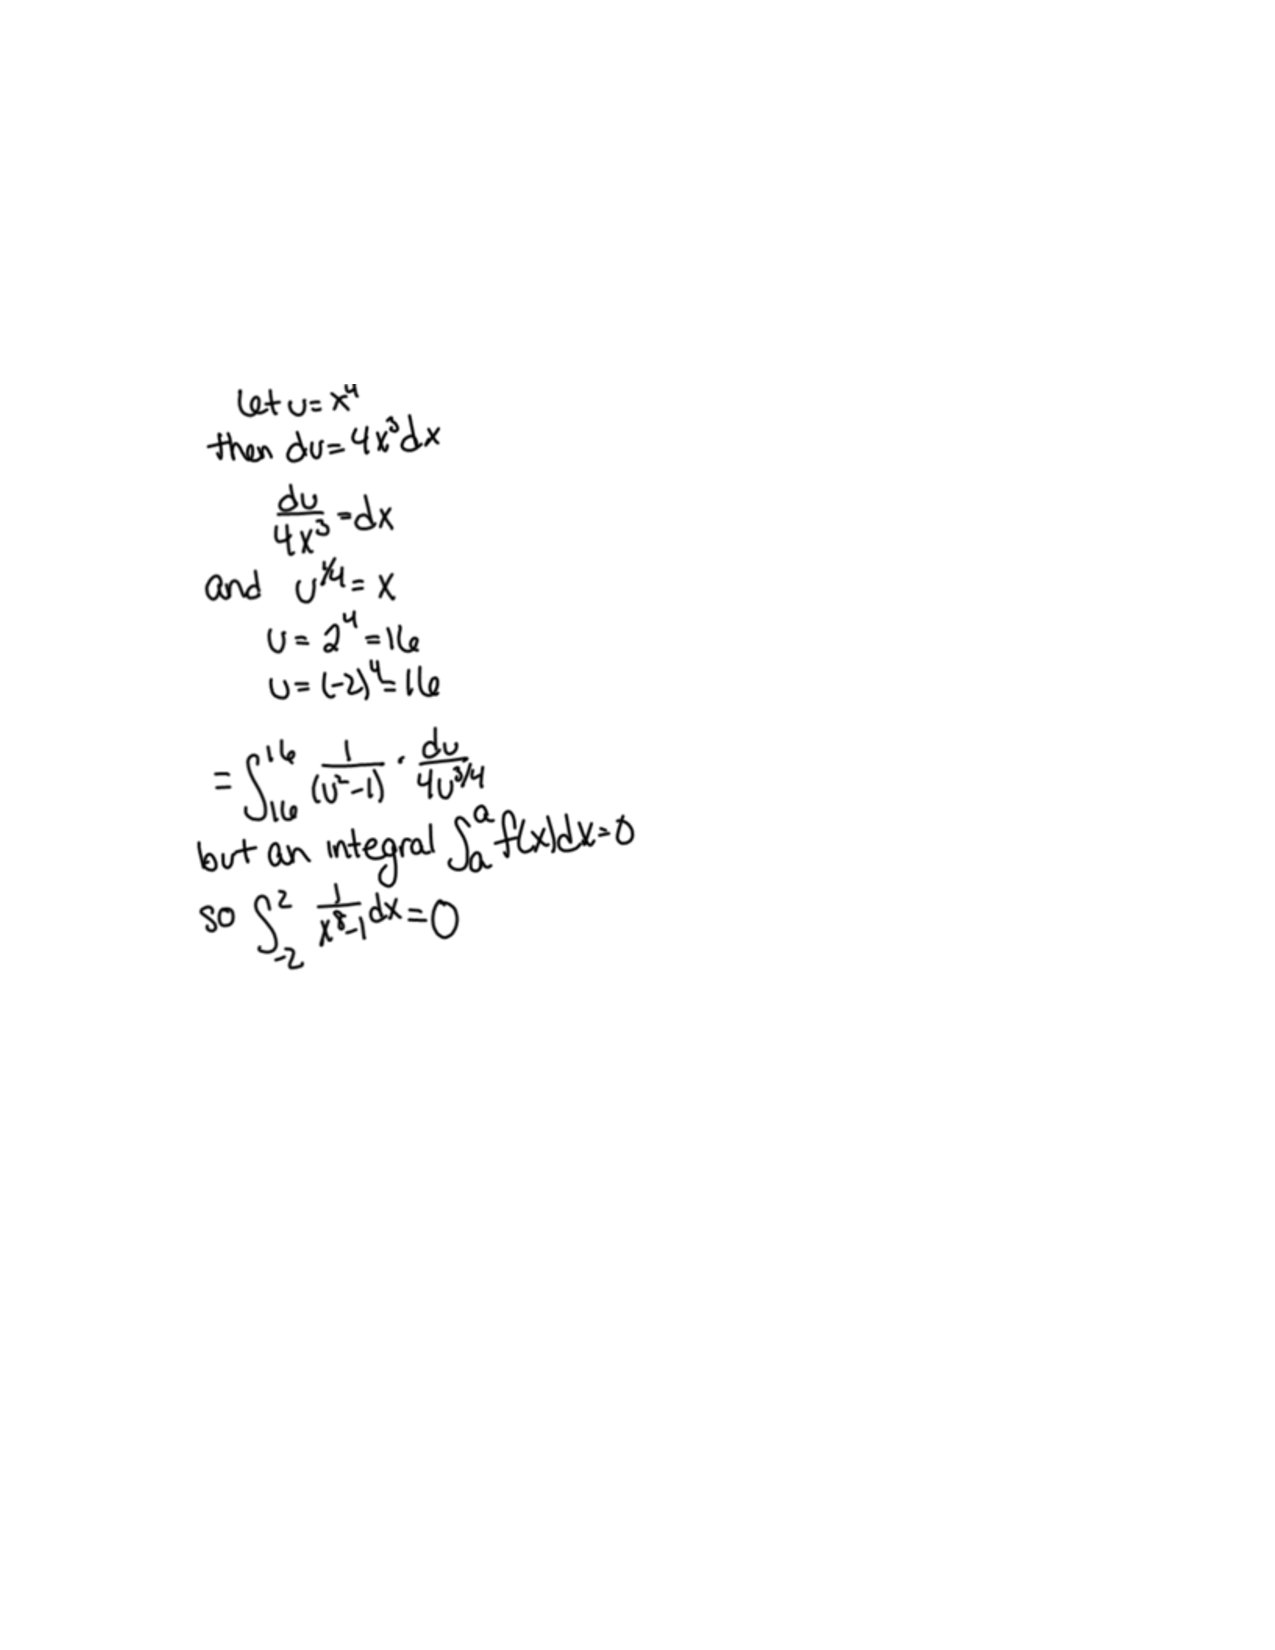
\includegraphics[trim= 170 420 250 180]{Figure1.pdf}
%\end{image}

%add a ``.'' below when used in a specific directory.
\newcommand{\RR}{\mathbb R}
\renewcommand{\d}{\,d}
\newcommand{\dd}[2][]{\frac{d #1}{d #2}}
\renewcommand{\l}{\ell}
\newcommand{\ddx}{\frac{d}{dx}}
\newcommand{\dfn}{\textbf}
\newcommand{\eval}[1]{\bigg[ #1 \bigg]}

\usepackage{multicol}

\renewenvironment{freeResponse}{
\ifhandout\setbox0\vbox\bgroup\else
\begin{trivlist}\item[\hskip \labelsep\bfseries Solution:\hspace{2ex}]
\fi}
{\ifhandout\egroup\else
\end{trivlist}
\fi} %% we can turn off input when making a master document

\title{Basic ideas of differential equations}  

\begin{document}
\begin{abstract}		\end{abstract}
\maketitle



\begin{comment}
\section{Warm up:}

	\begin{freeResponse}
	
	\end{freeResponse}
	
\begin{instructorNotes}

\end{instructorNotes}
\end{comment}







\section{Group work:}



%problem 1
\begin{problem}
Which of the following is a solution to the differential equation $y'' + 9y = 0$?
	\begin{enumerate}
	\item  $y=e^{3t}+e^{-3t}$
	\item  $y=C(t^2 + t)$
	\item  $y=\sin(3t) + 6$
	\item  $y=5 \cos(3t) - 7 \sin(3t)$
	\item  $y=A \cos(3t) + B \sin(3t)$ \text{ (where A and B are real numbers.)}
	\end{enumerate}
	\begin{freeResponse}
	
	\end{freeResponse}
	
\end{problem}

\begin{instructorNotes}
This is a good exercise in evaluating differential equations with functions.  
Suggest that each member in the group try a different possible solution.
\end{instructorNotes}







%problem 2
\begin{problem}
Verify that, if $y(0)=0$, that both $f(x)=1-(x^2+1)^2$ \dfn{and} $g(x) = 1 - (x^2-1)^2$ are solutions to the differential equation $\dd[y]{x} = 4x\sqrt{1-y}$.
	\begin{freeResponse}
	
	\end{freeResponse}
		
\end{problem}

\begin{instructorNotes}
Note that students will need to plug into both $x$ and $y$ in the differential equation.  
Also, make sure that students realize that an initial value problem can possibly have many solutions.
\end{instructorNotes}







%problem 3
\begin{problem}
Find a specific solution to the differential equation $\dd[y]{x} = x^{-2} \arctan(x)$ if $y(0)=5$.
	\begin{freeResponse}
	
	\end{freeResponse}

\end{problem}

\begin{instructorNotes}
This is a straight forward antiderivative problem.  
The real interest here is finding the antiderivative using integration by parts and then partial fractions.  
\end{instructorNotes}







%problem 4
\begin{problem}
Explain why the functions with the given graphs cannot be solutions of the differential equation $y' = e^x (y-1)^2$.
	%\begin{image}
	%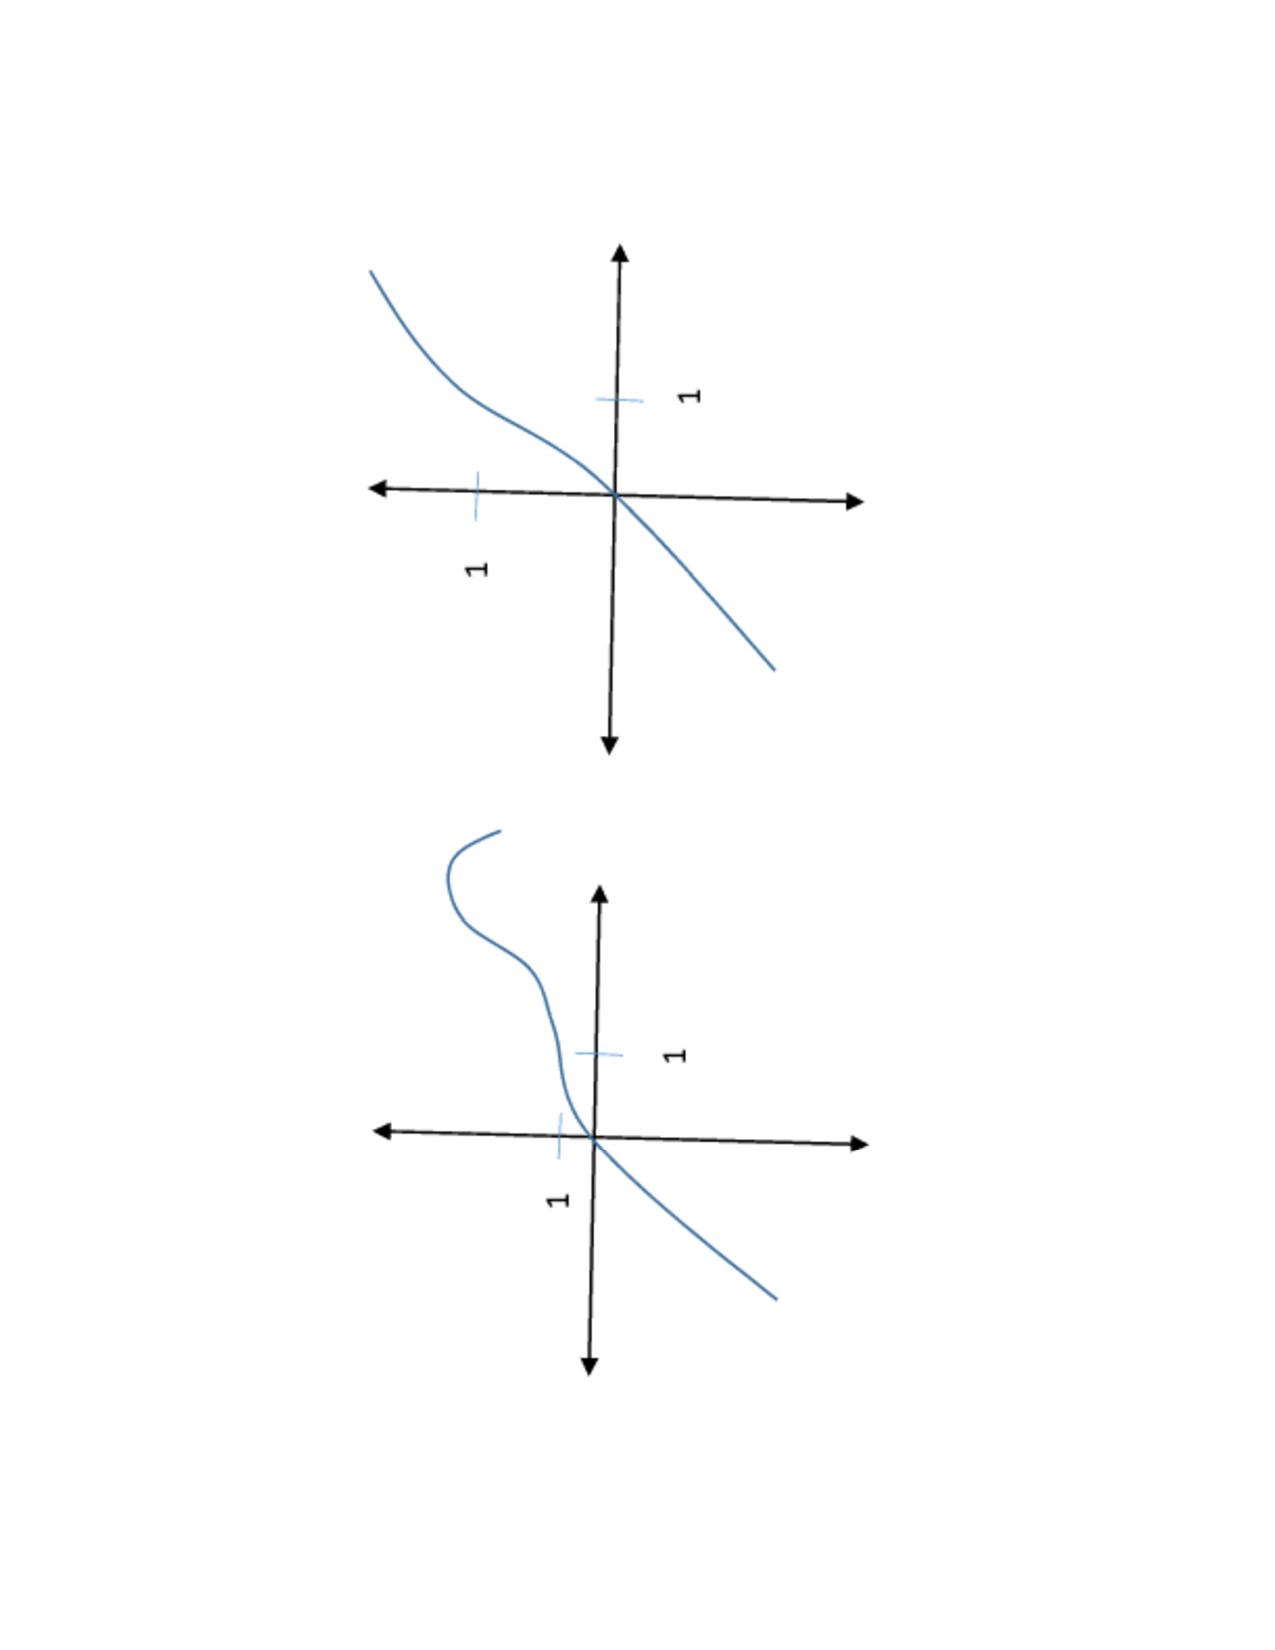
\includegraphics[trim= 170 420 250 180]{Figure8-1-1.pdf}	
	%\end{image}

	\begin{freeResponse}
	
	\end{freeResponse}

\end{problem}

\begin{instructorNotes}
This activity anticipates the idea of direction fields to be covered in Section 8.2.  
Students should eventually realize that differrential equations are statements about the slope of the function at each point $(x,y)$.  
Issues such as where the slope equals $0$ or where the slope is positive, negative, increasing, or decreasing should arise in the solution/discussion.  
The first graph has a negative slope at some places ($e^x$ and $(y-1)^2$ are always non-negative), and the second graph does not have a slope of $0$ at the point $(1,1)$.  
\end{instructorNotes}
















	
	
	
	
	
	
	
	
	

	










								
				
				
	














\end{document} 


















